\documentclass[11pt]{article}
\usepackage{framed, color}
\usepackage{textpos}
%\usepackage{natbib}
\usepackage{cite}
\usepackage[top=1in, bottom=1in, left=1in, right=1in]{geometry}
\usepackage{color}
\usepackage{hyperref}
\usepackage{textcomp}
\usepackage{graphicx}
\usepackage{fancybox}
\usepackage{setspace}
\hypersetup{colorlinks=false, urlcolor=blue, citecolor=black}
\usepackage{soul}
\usepackage{geometry}
\usepackage{color}
\newgeometry{top=1in, bottom=1in, left=1in, right=1in}
\usepackage{fancyhdr}
\usepackage{wrapfig}
\usepackage{mdframed}
\pagenumbering{arabic}
\usepackage[font=small,skip=0pt]{caption}


% Use the PLoS provided bibtex style
\bibliographystyle{plos2009}

\newcommand{\Drosophila}{\textit{Drosophila }}

\begin{document}

%\parindent 0.000000001in
\setlength{\parindent}{1cm}
\setcounter{page}{0}
\pagenumbering{arabic}

%The target of natural selection for behavior evolution is not just isolated actions, but extended sequence of behaviors driven by shifts in underlying motivational states \cite{Sibly:1976wq, scholes2006courtship}. Behavior often unfolds in a continuous stream, making motivational states corresponding to behavioral transitions difficult to discern, yet identification of these states is critical for understanding the mapping between genetic (e.g. in neuromodulatory systems) and behavioral variation \cite{Houston:1976wh}. 

\setcounter{page}{1}
\noindent \textbf{Background:} Understanding the targets of natural selection on behavior is challenging in large part because behavior consists not just of isolated actions, but as extended sequence of actions driven by shifts in underlying motivational states \cite{Sibly:1976wq, scholes2006courtship}. Discerning the motivational states corresponding to behavioral transitions is difficult because behavior unfolds in a continuous stream, and yet identification of these states is critical for understanding the mapping between genetic (e.g. in neuromodulatory systems) and behavioral variation \cite{Houston:1976wh}. One way to address this is the use of Hidden Markov Models (HMM).  HMMs use any kind of �sequence data� (or transition matrices derived from sequence data) to estimate latent (hidden) variables, with transitions between hidden states influencing observed behavioral states (emission probabilities).  HMMs are used in image processing, text processing, bioinformatics (gene finding) as well as for the study of behavior \cite{feldman2004representing, Krogh:1998vm, Rimey:1991gi,Morgan:1976tv, stanke2003gene, eddy1998profile, rabiner1989tutorial, brand1997coupled}. With respect to the study of behavior, the �hidden� variables are often used to model underlying motivational states \cite{Zucchini:2008tw, MacDonald:1995bu, Carola:2011ei, Patterson:2009bc}. Importantly, HMMs allow for the incorporation of additional predictors and hierarchical structure to assess biological factors (sex, species) and reduce assumptions (stationarity and homogeneity) that have plagued other forms of sequential analysis. Exciting recent development of random effects HMMs \cite{Altman:2007ix, Maruotti:2011jt, Zucchini:2008tw, SchlieheDiecks:2012fc} may allow for the rigorous evaluations of questions pertaining to behavioral syndromes (personality), yet such extensions have not yet been realized nor implemented in a general framework.

Despite the potential of HMMs, the meaning of the hidden (latent) states is rarely obvious. Currently it is unclear how the �hidden� factors can be interpreted as motivational or neurophysiological states. Thus in addition to issues of estimation and inference inherent in all data modeling approaches, whether HMMs lead to biologically relevant inferences about underlying mechanisms is unclear. Evaluation of hidden factors in contexts like gene finding is relatively easily (detecting transcripts or gene function), but is less straightforward for behavior. Thus there is a critical need to both extend and evaluate HMMs in systems where motivational states can be directly evaluated, and thereby to correlate latent variables in HMMs to validated control mechanisms.\\

\begin{wrapfigure}{r}[0pt]{0.54\textwidth}
\hypertarget{Figure 1}{}
\vspace{-10mm}
\begin{mdframed}
  \begin{center}
    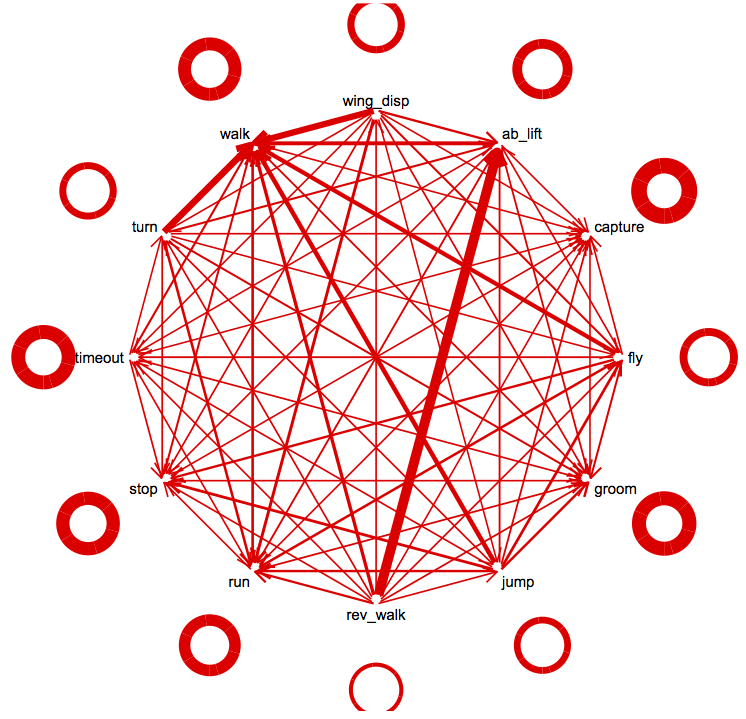
\includegraphics[width=1\textwidth]{Spider_tmatrix2.png}
  \end{center}
   \setlength{\abovecaptionskip}{0cm}
   \caption{\scriptsize{Transition probabilities for \Drosophila behaviors in the presence of a predator. Arrow/circle thickness depicts observed transitions/time in state.}}
\end{mdframed}
\end{wrapfigure}

\noindent \textbf{Objectives:} The long term goal of this research is to understand the evolution of underlying motivational states, and observed sequence of behaviors. This proposal seeks to extend and evaluate the suitability of HMMs to address such questions, using a two-stage interdisciplinary strategy. We will use behavioral sequence data from several biological systems (where motivational states can be experimentally manipulated through the presentation of biologically meaningful stimuli) and from Avida, where we can directly examine the underlying execution of operations leading to the observed behaviors. This research will have implications for the study of behavioral sequence analysis specifically as well as Hidden Markov Models more generally. In particular, we expect to explore methods for validating the biological traits corresponding to latent variables detected by HMMs as well as extending HMMs to incorporate random effects (i.e personality) and hierarchical structures.\\

\noindent \textbf{Aim 1:} \emph{Extend and evaluate the interpretability of HMMs for underlying motivational states in behavioral analysis using Avida.}\\

\noindent \textbf{Aim 2:} \emph{Evaluate motivational states in biological systems (\Drosophila and bees) where these can be manipulated via evolutionary or experimental manipulations.}

\begin{center}
\textsc{{Proposed Research}} \\
\end{center}

\noindent \textbf{Aim 1:} We will set up simplified experiments with focal Avidians. Utilizing a cross-section of Avida organisms evolved during previous experiments on foraging strategies \cite{bartlettEvolution}, and predation and predator-avoidance behaviors \cite{wagner2013arms}, we will record both their realized behavioral sequences and the actual execution order (trace) of their genetic programs.  We will analyze these genetic programs with their execution traces to identify the sensory inputs and internal states that were used in formulating decisions.  We will also feed the behavioral sequences produced into HMM generators to measure the number of internal states predicted by the HMM, and how each influence behavior.  This phase of research will enable us to determine the correspondence of estimated HMMs with the actual control system used by the digital organisms, allowing calibration of our HMM estimation techniques to maximize correspondence for use in the subsequent aims. In addition this will allow us to evaluate how estimation is influenced by important empirical parameters such as time allotted to observations, number of observed states, and number of observed transitions.\\


\begin{wrapfigure}{r}[0pt]{0.4\textwidth}
\hypertarget{Figure 2}{}
\vspace{-7mm}
\begin{mdframed}
  \begin{center}
    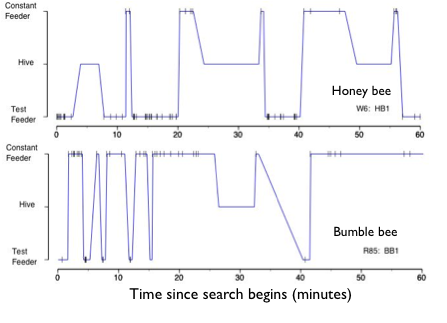
\includegraphics[width=1\textwidth]{FD_v1.png}
  \end{center}
   \setlength{\abovecaptionskip}{0cm}
   \caption{\scriptsize{Behavioral transitions of two individual bees (of different species) during search.}}
\end{mdframed}
\end{wrapfigure}

\noindent \textbf{Aim 2:} While behavioral sequence data is widely available, rarely are the inferred motivational states explicitly validated by evidence for the proximate mechanisms of state transitions. We will use the primary systems of Dworkin and Dyer, namely searching behavior in bees and anti-predator behaviors in \Drosophila. As seen in \hyperlink{Figure 1}{Figure 1}, \Drosophila exhibit a wide array of behaviors in the presence of predators \cite{Parigi:vg}, with non-random transitions between them.  We will manipulate predation risk to alter underlying motivational states in populations evolved with and without a predator (zebra jumping spider) for $\sim$60 generations. Dyer will use both previously collected and new data to address the underlying motivational states in two species of bees. Prior work has shown that experiencing changes in the quality and amount of food alters behavioral sequences related to the learning of new resources \cite{wei2009investing, wei2002deciding} or searching for resources not yet found. This occurs in a species specific manner \cite{townsend2011deciding,townsend2012integrated}.  \hyperlink{Figure 2}{Figure 2} shows data from two bees of different species as they search without reward among three locations over the course of an hour. We will investigate whether an HMM approach can explain behavioral sequence variation involving changes in some hidden states independent of others or if states are modulated in a correlated way. This may guide future work exploring gene expression dynamics for genes known to modulate foraging behavior in insects.

We will use several libraries in \textsc{r}  (\textsc{depmixs4, HiddenMarkov, HMM, hmm.discnp, RHmm}) and Python (\textsc{ghmm wrapper, scikit-learn, hmmpytk, pyhmmtb}) to assess performance of the HMMs. As there is no general purpose software for hierarchical or random effect HMMs \cite{Altman:2007ix, Maruotti:2011jt, Zucchini:2008tw,SchlieheDiecks:2012fc}, PI Dworkin will prototype them in the \textsc{stan} probabilistic programming language for hierarchical modeling using MCMC \cite{stan-software:2013, hoffman-gelman:2013}. A general purpose parser will be written to generate files in appropriate input formats.


\newpage
\setcounter{page}{1}
\thispagestyle{empty}
\singlespacing
%\bibliographystyle{model2-names.bst} % for natbib
\bibliography{HMM_refs.bib}


\end{document}
